%priprava posamezne ure
%tukaj zaporedoma napisemo{st. zaporedne ure}{datum}{naslov}{poglavje}{oblika dela}{pripomocki}
\begin{priprava}{}{}{Integral}{Določeni integral}{frontalna}{tabla}

\didopomba{Začnemo z nečim, kar na prvi pogled nima veze z integralom.}

\naslov{Geometrijski pomen}

Koliko je ploščina območja, ki ga funkcija $ f(x) = x - 1 $ na intervalu $ [2, 4] $ oklepa z $ x $-osjo? \didopomba{Izračunamo iz slikce preko trikotnika in pravokotnika (4).}

\begin{figure}[h]
    \centering
    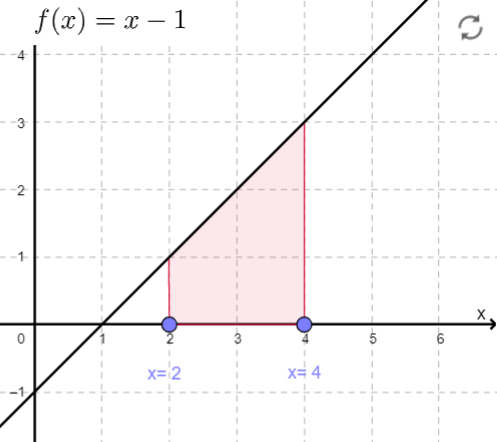
\includegraphics[width=0.4\textwidth]{slike/dol_int_motivacijski_primer.png}
\end{figure}

\didopomba{Zdaj pa si pogledamo \href{https://www.geogebra.org/m/Fv6t696j}{aplet na Geogebri}, v zvezek si bomo risali potem.} Vzamemo drugačno funkcijo: $ f(x) = \sin{2x}+\frac{x^2}{10} + 1 $ na intervalu $ [1,5] $. Kako bi izračunali ploščino pod grafom?

\begin{figure}[h]
    \centering
    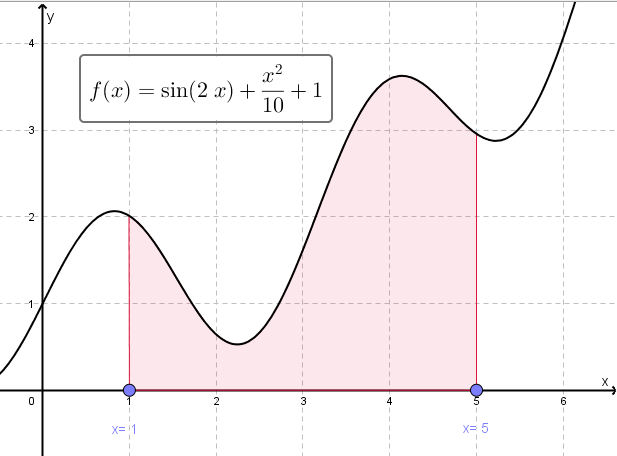
\includegraphics[width=0.3\textwidth]{slike/dol_int_motivacijski_primer2.png}
    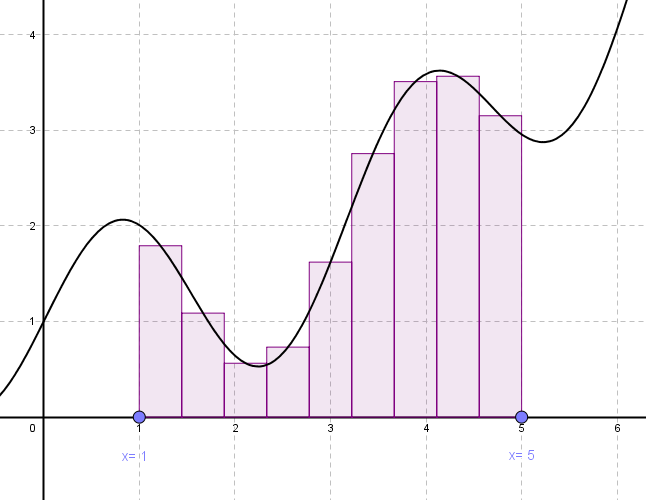
\includegraphics[width=0.3\textwidth]{slike/midpoint.png}
    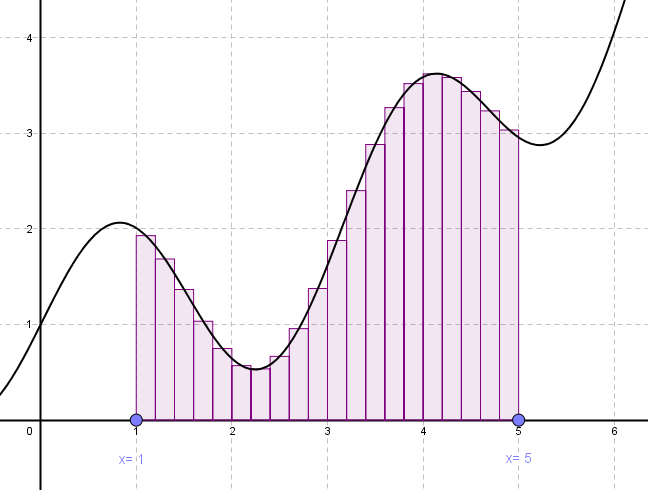
\includegraphics[width=0.3\textwidth]{slike/midpoint2.png}    
\end{figure}


\didopomba{Naj sami predlagajo, da območje razdelimo na znane like, pravokotnike, recimo z enako širino -- ampak s kakšno višino?}

\didopomba{Interval razdelimo na enako široke podintervale. Na vsakem pointervalu si izberemo točko, in vrednost funkcije $ f $ v tej točki bo višina pravokotnika na tem podintervalu. Lahko si izberejo levo/desno mejo podintervalov, ali točko, kjer $ f $ na podintervalu doseže maksimum/minimum, recimo da mi vzamemo kar točke na sredini podintervalov.}

\didopomba{Iz animacije vidimo: če interval razdelimo na večdno več delov, se pravokotniki ožajo in se njihova vsota ploščin približuje iskani ploščini.}

\didopomba{Zdaj pa pišemo/rišemo v zvezek (splošna $ f $ na $ [a, b] $).}

\newpage

Ploščino lahko zapišemo kot vsoto ploščin $ n $ pravokotnikov s širino $ \Delta x $ in višino $ f(x_i) $, kjer so $ x_i $ sredinske točke $ i $-tega podintervala $ [a, b] $ \didopomba{izkaže se, da so to lahko katerekoli točke iz intervala}.

$$ S_n = \sum_{i=1}^n f(x_i) \cdot \Delta x \text{ \didopomba{to je vijola ploščina}}$$

\begin{figure}[h]
    \centering
    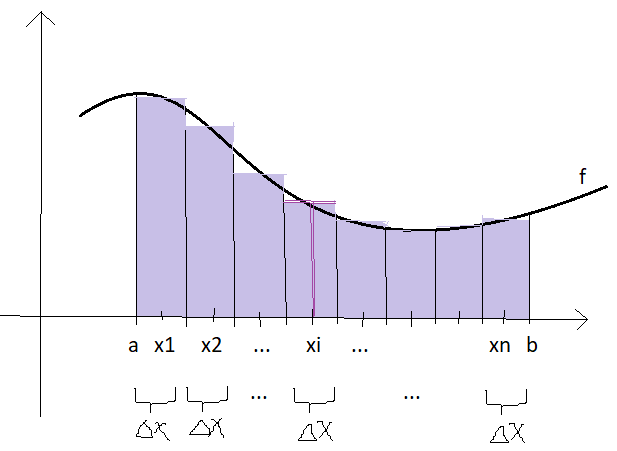
\includegraphics[width=0.65\textwidth]{slike/dol_int_skica0.png}
\end{figure}

Več je podintervalov, bolj se vsota ploščin pravokotnikov približuje pravi ploščini \didopomba{torej bo govora o limiti}.

\didopomba{Limito te vsote označimo z znakom $ \int $ (oznako je uvedel Leibniz); integral je v bistvu ena vsota, kjer se pomikamo po res neskončno majhnih korakih. Pri tem se $ \Delta x $ zamenja z $ dx $, s čimer poudarimo, da gredo širine podintervalov res proti 0.}

$$
S = \lim_{n \rightarrow \infty} \sum_{i=1}^n f(x_i) \cdot \Delta x = \int_a^b f(x) dx
$$

$ a $ imenujemo \textbf{spodnja meja} integrala, $ b $ pa \textbf{zgornja meja}.

\didopomba{Od \underline{tu} pride oznaka $ \int dx $ pri nedoločenih integralih, ne pa obratno. Zakaj pa smo se učili nedoločene integrale, pa še pridemo do tega ... Poudari, da je dol. integral število (ne pa funkcija)! Zaenkrat ga še ne znamo izračunati, še pride. KJE JE POVEZAVA? ŠE PRIDE PRI N-L FORMULI, BOJO ŽE VIDLI, POTEM SE VSE POKLOPI!}

Če je $ f (x) $ na $ [a, b] $ zvezna in nenegativna, je \textbf{Določeni integral $ \int_a^b f(x) dx $ enak ploščini lika, ki je omejen z grafom funkcije $ f $, $ x $-osjo ter premicama $ x = a $ in $ x = b $.}

\begin{figure}[h]
    \centering
    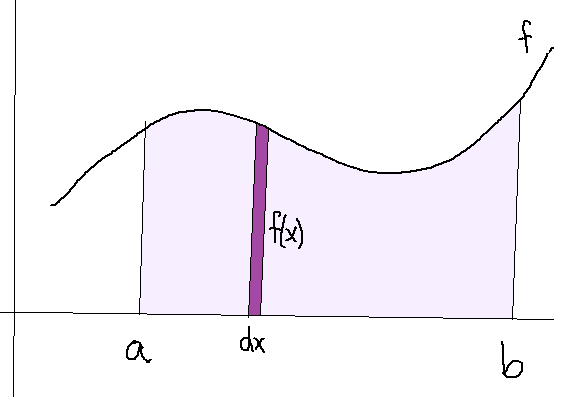
\includegraphics[width=0.4\textwidth]{slike/dol_int_skica.png}
\end{figure}

\newpage

\didopomba{Za zvezno lahko pokažeš, da odsekoma zvezne funkcije ne moreš sploh vpisat v integral. Za negativno pa upoštevaš, da je $ f(x_i) < 0 $, torej je vsota $ \sum f(x_i) \Delta x $ negativna in s tem tudi  integral negativen. Ploščina pa je po velikosti seveda enaka (spodnja slika)}.

\begin{figure}[h]
    \centering
    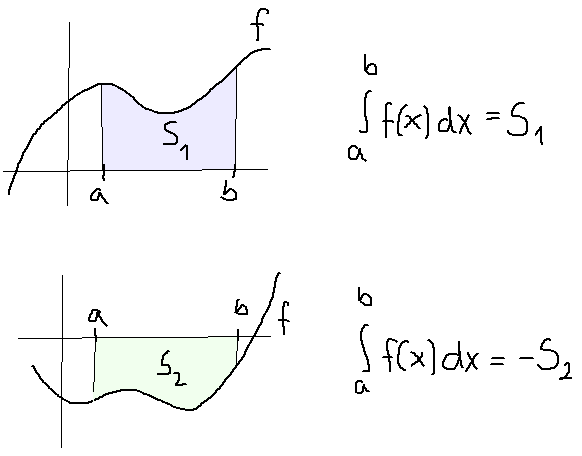
\includegraphics[width=0.6\textwidth]{slike/ploscine.png}
\end{figure}

Kaj pa, če je na $ [a, b] $ funkcija malo pozitivna, malo negativna?

\begin{figure}[h]
    \centering
    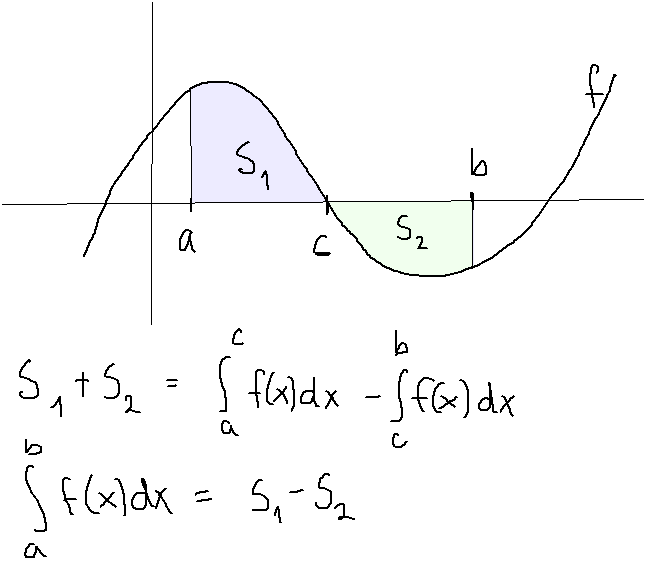
\includegraphics[width=0.5\textwidth]{slike/ploscine2.png}
\end{figure}

Ploščina območja je tako vedno enaka $ S = \int_a^b | f(x) | dx $ ne glede na predznak $ f $.

\vaje{Kratka vaja (npr. slikco s polinomom z znanimi ploščinami, zaenkrat računaš le po eno območje naenkrat, pač enkrat bo +, enkrat -)}:

\begin{figure}[h]
    \centering
    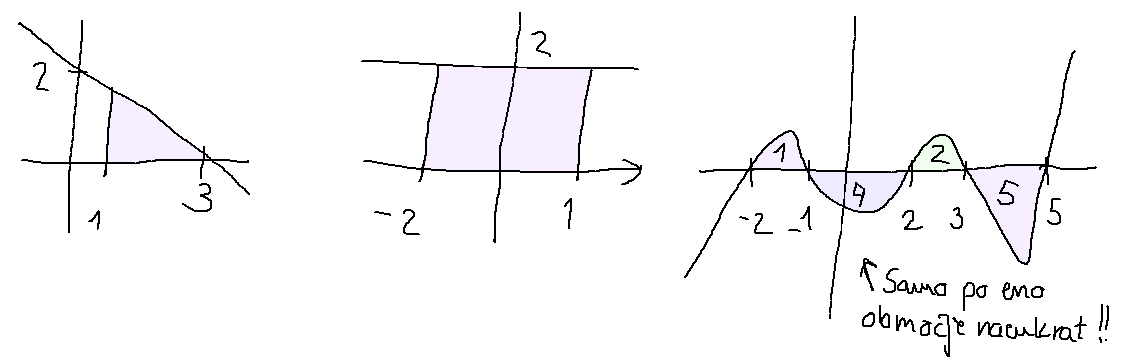
\includegraphics[width=0.9\textwidth]{slike/dol_vaje1.png}
\end{figure}

\newpage

Potem pa še nekaj logičnih lastnosti \didopomba{sledijo iz ploščine (lahko zraven skice), se jih tudi preveri, ko spoznajo N-L formulo}:

\naslov{Lastnosti}

\begin{itemize}
    \item $ \int_a^a f(x) dx = 0 $
    \item $ \int_a^c f(x) dx + \int_c^b f(x) dx = \int_a^b f(x) dx $, kjer je $ c \in [a, b] $
    \item $ \int_a^b f(x) dx = - \int_b^a f(x) dx $ \didopomba{To je bolj dogovor, ampak bo pa očitno sledilo iz NL formule}
    \item $ \int_a^b c \cdot f(x) dx = c \cdot \int_a^b f(x) dx $
    \item $\int_a^b (f(x) + g(x)) dx = \int_a^b f(x) dx + \int_a^b g(x) dx $
    \item Izrek o povprečni vrednosti: $ \int_a^b f(x) dx = (b-a)p \rightarrow $: $ p = \frac{1}{b - a} \int_a^b f(x) dx $
        \begin{figure}[h]
            \centering
            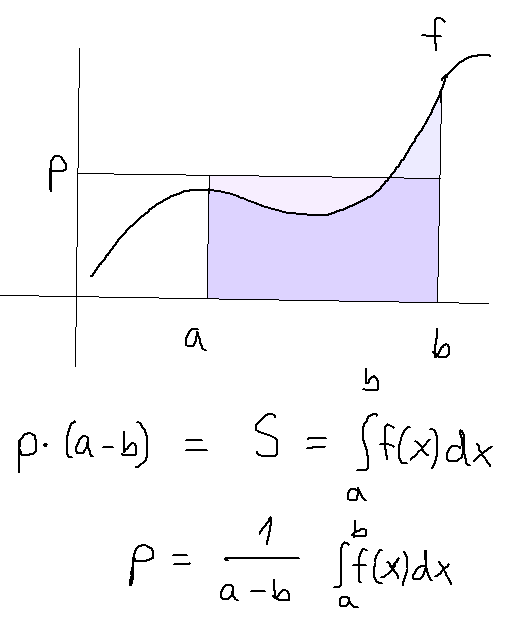
\includegraphics[width=0.4\textwidth]{slike/povprecna_vrednost.png}
        \end{figure}
\end{itemize}

\vaje{
Vaje:
\begin{itemize}
    \item Lahko naloge -- funckije z znano ploščino (jo znaš razbrati iz grafa, kakšne premice, absolutno, krožnice ...), najprej na enem območju, pozitivno/negativno, nato oboje ipd.
    \item funkcije,, ki se ne da enostavno ploščine izraziti, ampak se ploščine odštejejo v 0 (npr. lihe funkcije, $ \int_0^{2\pi} \sin x dx $)
    \item sode funkcije na simetričnem intervalu $ [-a, a] $ -- lahko integriraš po $ [0, a] $ in podvojiš! (včasih je to enostavneje, saj vstavljaš v eno mejo 0).
    \subitem tudi $ \int_{-\pi/2}^{pi/2} \cos x dx $ je vredu primer, pač se da poenostavit v $ \int_0^{\pi/2} \cos x dx $.
    \item valovita funkcija z odsekoma znanimi ploščinami (ampak neznanim predpisom) in morajo izračunati določeni integral na različnih intervalih, pa $ 2f(x), -f(x), |f(x)| $ ipd.
    \item Oceni ploščino funkcije (npr. na [0, 2], min = 1 in max = 2 -> ploščina je med 2 in 4. Nato jo še izračunamo.)
\end{itemize}
}

\newpage

Zdaj pa nam že malo nagaja, ker ne znamo izračunati določenega integrala, npr. drugega primera ($ f(x) = \sin{2x}+\frac{x^2}{10} + 1 $) ne znamo izračunati ...

\naslov{Newton-Leibnizova formula}

Da bomo lahko integral lahko tudi izračunali, si za začetek poglejmo funkcijo na sliki (levo) \didopomba{čim manj piši, lahko le s puščicami povežeš slikce in formule}, ki jo definiramo s \didopomba{$ s < a $ ni važen}:

$$ F(x) = \int_s^x f(t) dt $$

\begin{figure}[h]
    \centering
    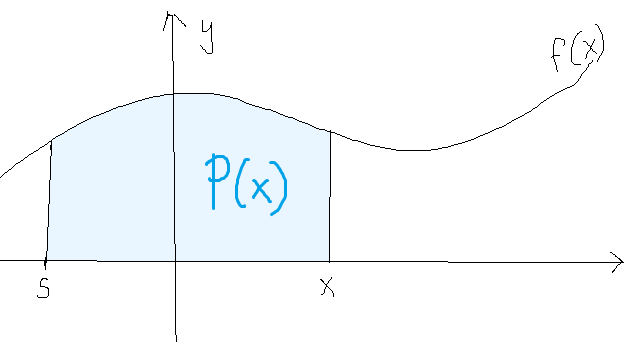
\includegraphics[width=0.45\textwidth]{slike/NL_P(x).png}
    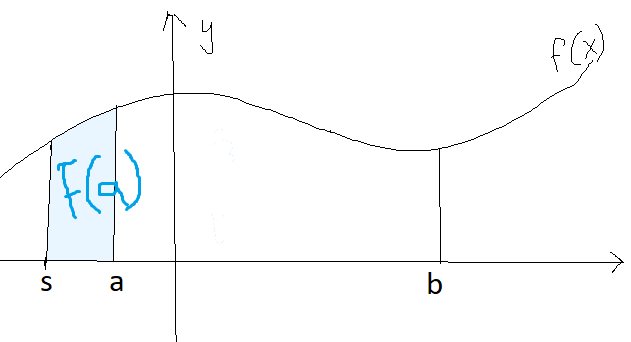
\includegraphics[width=0.45\textwidth]{slike/NL_P(a).png}
\end{figure}

\begin{figure}[h]
    \centering
    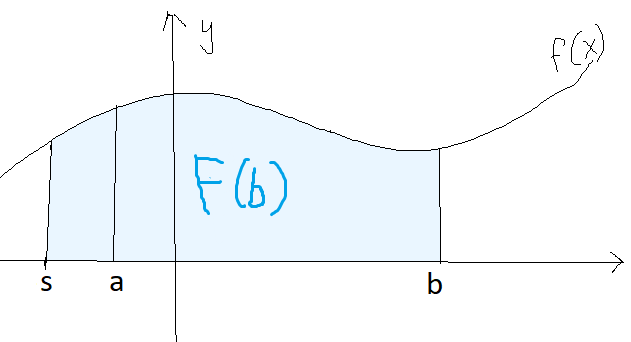
\includegraphics[width=0.45\textwidth]{slike/NL_P(b).png}
    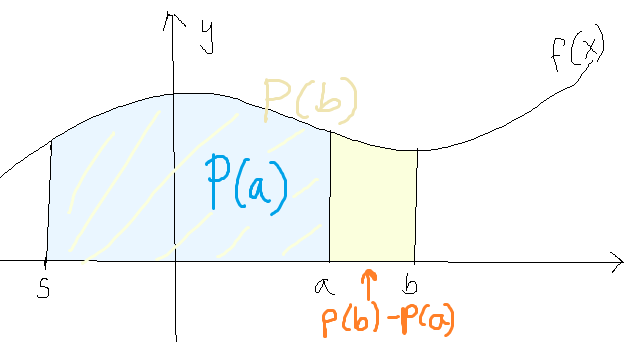
\includegraphics[width=0.45\textwidth]{slike/NL_P(b)-P(a).png}
\end{figure}

Iz slik opazimo, da velja

$$ \int_a^b f(x) dx = F(b) - F(a) $$

Super, kako pa izračunamo F? Poglejmo si njen odvod po definiciji \didopomba{pomoč s spodnjo slikco, višina tega ``pravokotnika'' je v limiti kar $ f(x) $}:

$$
F'(x) = \lim_{h \rightarrow 0} \frac{F(x + h) - F(x)}{h} = \lim_{h \rightarrow 0} \frac{f(x) \cdot h}{h} = f(x)
$$

\begin{figure}[h]
    \centering
    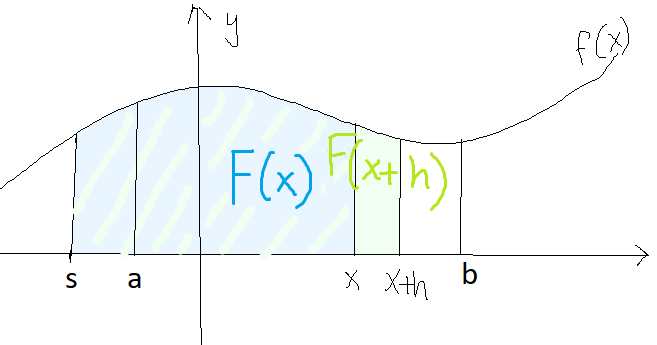
\includegraphics[width=0.5\textwidth]{slike/NL_P(x)_P(x+h).png}
\end{figure}

\newpage

Že vemo, da $ F'(x) = f(x) $ pomeni, da je $ F(x) $ nedoločen integral funkcije $ f $ \didopomba{torej že znamo izračunati $ F $} in to je to. \didopomba{Tukaj se zdaj vse poklopi skupaj -- nedoločen intergral, ploščine in določen integral}


Povzemimo: če je funkcija $ F(x) $ nedoločen integral funkcije $ f(x) $, potem velja:

\begin{align*}
    \int f(x) dx & = F(x) + c \text{ \didopomba{to že vemo}} \\
    \textcolor{rdeca}{\int_a^b f(x) dx} & = \textcolor{modra}{F(x)|_a^b} \textcolor{rdeca}{= F(b) - F(a)} \\
    \text{ \textbf{Newton}} & \text{\textbf{-Leibnizova formula (NL-formula).}}
\end{align*}

\didopomba{Oznako s $ | $ napiši nazadnje, pač to je krajši zapis. Tu ni več c-jev, ker se odštejejo!}

Z besedo: \emph{Določen integral funkcije je enak razliki vrednosti njenega nedoločenega integrala na zgornji in spodnji meji.}

Izračunamo prav ta prvi primer pri določenem integralom še s to formulo: $ \int_2^4 (x - 1) dx = (\frac{x^2}{2} - x) |_2^4 = 4 $.

Pa še drugega: $ \int_1^5 (\sin{2x}+\frac{x^2}{10} + 1) dx = \ldots \approx 8,14 $

\vaje{
Vaje:
\begin{itemize}
    \item Z N-L formulo preveri veljavnost pravil, ki smo jih našteli zgoraj \didopomba{razen povprečne vrednosti}
    \item basic vaje
    \item odsekoma zvezna funkcija \didopomba{Sami pogruntajo, da morajo ločiti na vsoto več integralov}
    \item Za integral $ \int_e^{e^2} \ln x dx $ ugotovi, ali je večji od 2, ali je večji od 30. \didopomba{Naj sami razmislijo, kako se tega lotiti.}
\end{itemize}
}

\naslov{Per partes v nedoločenem integralu}

A je to sploh noter? Sicer pa itak sam dodaš meje.

\naslov{Uvedba nove spremenljivke}

\textcolor{rdeca}{PAZI! Le če je nova spremenljivka monotona funckija, lahko to narediš !! (sicer se ti vmes integral malo odšteje/prišteje \ldots)}

$ \int_1^3 (2x + 1)^5 dx $ lahko rešimo na dva načina:
\begin{itemize}
    \item kot do sedaj (izračun nedoločenega integrala): $ \int (2x + 1)^5 dx = \int \frac{t^5}{2} dt = \frac{(2x + 1)^6}{12} + c $
    \subitem $ \int_1^3 (2x + 1)^5 dx = \frac{(2x + 1)^6}{12} |_1^3 = \ldots = \frac{29230}{3} $
    \item s spremembo meje: $ \int_1^3 (2x + 1)^5 dx = \int_3^7 \frac{t^5}{2} dt = \frac{t^6}{12} |_3^7 = \frac{29230}{3} $
\end{itemize}
\didopomba{Nazorno zapiši pri mejah $ 2 \cdot 1 + 1 = 3 $ itd.}

\vaje{Vaje: Spet nekaj primerov za zamenjavo spremenljivk.}

\end{priprava}